
\subsection{Kiểm thử và kết quả mô phỏng hệ thống nâng cao}

\subsubsection{Sơ đồ mạch RTL (RTL Schematic)}
Sau khi tổng hợp toàn bộ hệ thống nâng cao trên phần mềm Vivado, sơ đồ mạch RTL được tạo ra giúp xác thực cấu trúc kết nối phần cứng.

\begin{figure}[H]
    \centering
    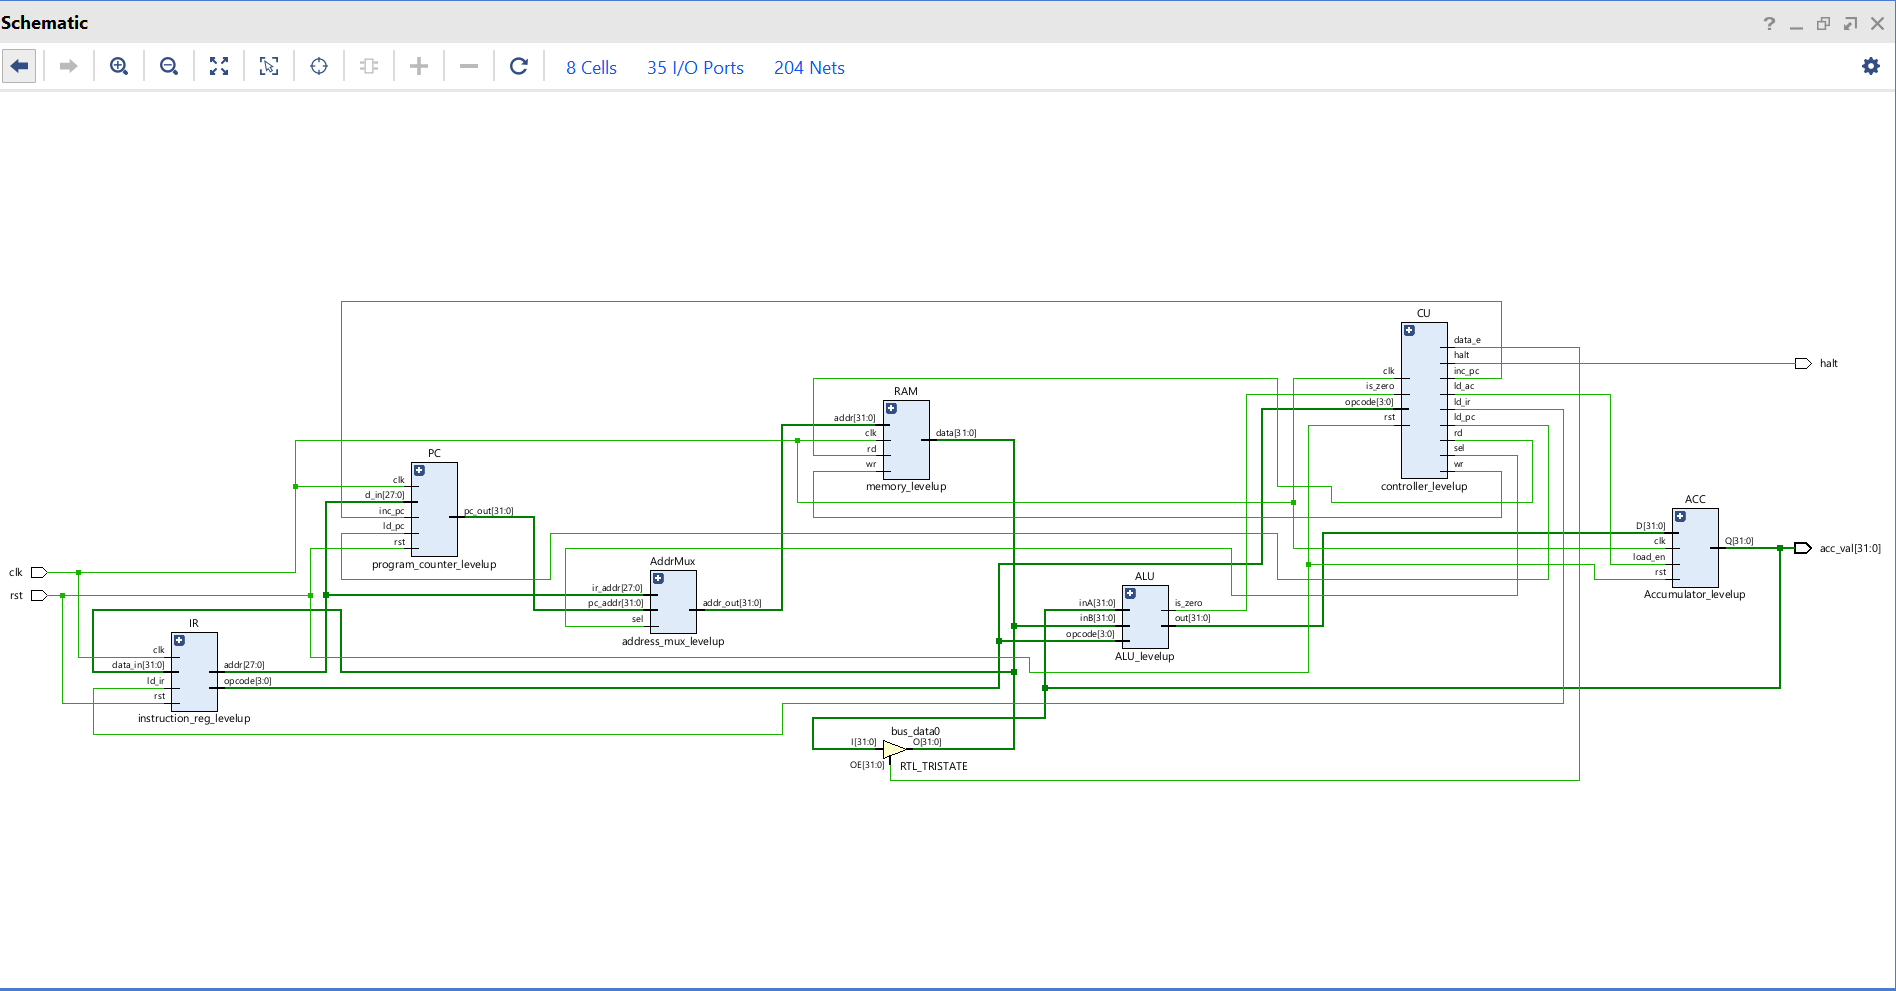
\includegraphics[width=1.0\textwidth]{sodo.png} 
    \caption{Sơ đồ mạch tích hợp hệ thống CPU nâng cao (RTL Schematic)}
    \label{fig:rtl_schematic_75}
\end{figure}

Sơ đồ RTL xác nhận toàn bộ 7 khối chức năng đã được kết nối chính xác theo kiến trúc thiết kế. Một số điểm kỹ thuật đáng lưu ý:
\begin{itemize}
    \item \textbf{Cơ chế Bus:} Khối \texttt{RTL\_TRISTATE} tại \texttt{bus\_data} đảm bảo dữ liệu từ Accumulator chỉ được đẩy lên bus khi tín hiệu $data\_e = 1$.
    \item \textbf{Mở rộng Opcode:} Đường tín hiệu \texttt{opcode[3:0]} (4-bit) kết nối trực tiếp giữa IR, ALU và Controller.
    \item \textbf{Tài nguyên:} Hệ thống sử dụng 8 Cells, 35 I/O Ports và 204 Nets, phản ánh quy mô của CPU 32-bit nâng cao.
\end{itemize}

\subsubsection{Mã kiểm thử hệ thống (Testbench)}
Đoạn mã Testbench dưới đây thực hiện nạp các giá trị vào RAM và thực thi chuỗi lệnh để kiểm tra các tính năng mới như \textbf{SUB} và \textbf{SHL}.

\begin{lstlisting}[caption={Mã Testbench cho CPU nâng cao}, label={lst:tb_75}]
`timescale 1ns / 1ps
module tb_CPU_levelup();
    reg clk; reg rst;
    wire halt; wire [31:0] acc_val;

    CPU_Top_levelup uut (
        .clk(clk), .rst(rst), .halt(halt), .acc_val(acc_val)
    );

    always #5 clk = ~clk;

    initial begin
        clk = 0; rst = 1;
        // Nap du lieu vao RAM
        uut.RAM.ram[10] = 32'd15;  
        uut.RAM.ram[11] = 32'd5;   
        uut.RAM.ram[12] = 32'd10;  

        // Nap chuong trinh
        uut.RAM.ram[0] = 32'h5000000A; // LDA 10 -> AC=15
        uut.RAM.ram[1] = 32'h2000000B; // ADD 11 -> AC=20
        uut.RAM.ram[2] = 32'h90000000; // SHL    -> AC=40
        uut.RAM.ram[3] = 32'h8000000C; // SUB 12 -> AC=30
        uut.RAM.ram[4] = 32'h6000000D; // STO 13
        uut.RAM.ram[5] = 32'h00000000; // HLT

        #15 rst = 0; 
        wait(halt == 1'b1);
        $finish;
    end
endmodule
\end{lstlisting}

\subsubsection{Giản đồ thời gian (Waveform)}
Quá trình tính toán được thể hiện chi tiết qua các chu kỳ xung nhịp trong giản đồ sóng:

\begin{figure}[H]
    \centering
    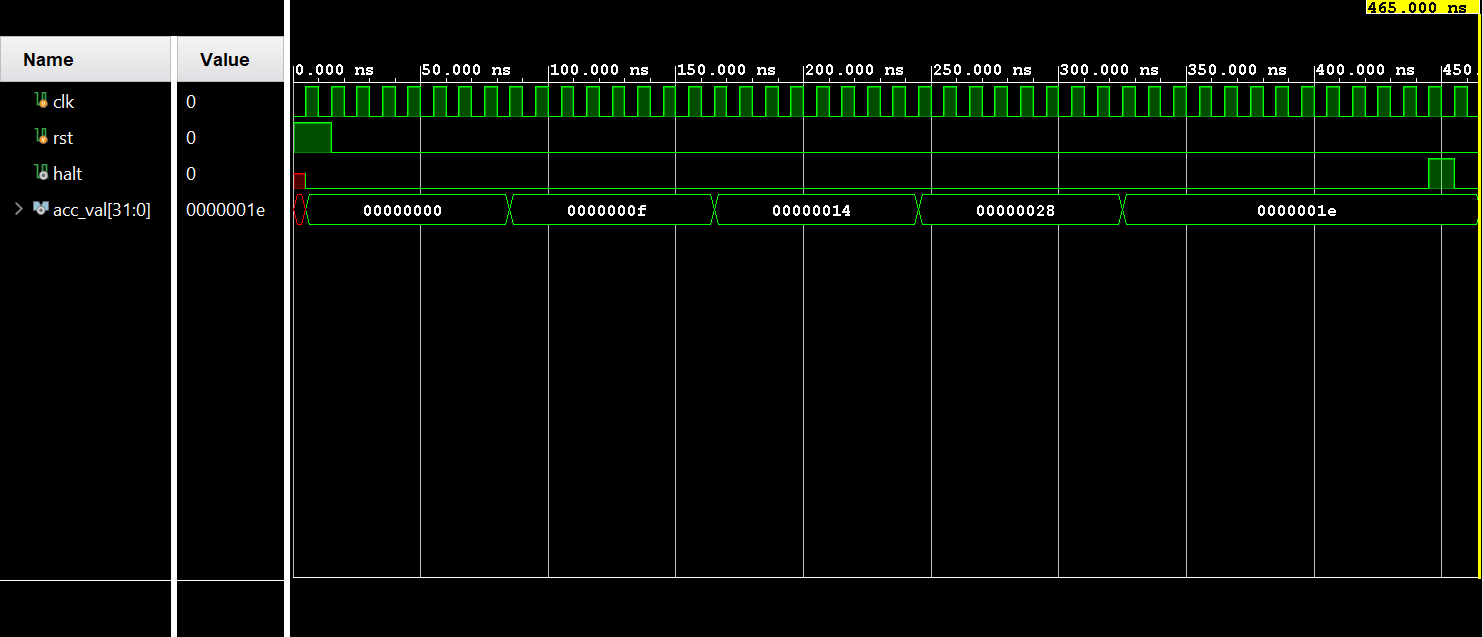
\includegraphics[width=1.0\textwidth]{wave.png} 
    \caption{Giản đồ thời gian mô phỏng CPU nâng cao}
    \label{fig:waveform_75}
\end{figure}

Logic toán học được thực thi qua các giai đoạn như sau:
\begin{enumerate}
    \item $ACC = RAM[10] = 15$
    \item $ACC = 15 + 5 = 20$
    \item $ACC = 20 \ll 1 = 40$ (Lệnh dịch trái SHL)
    \item $ACC = 40 - 10 = 30$ (Lệnh trừ SUB)
\end{enumerate}

\subsubsection{Kết quả xuất ra màn hình (Console Output)}
Kết quả kiểm thử cuối cùng được in ra cửa sổ Tcl Console xác nhận tính đúng đắn của toàn bộ hệ thống.

\begin{figure}[H]
    \centering
    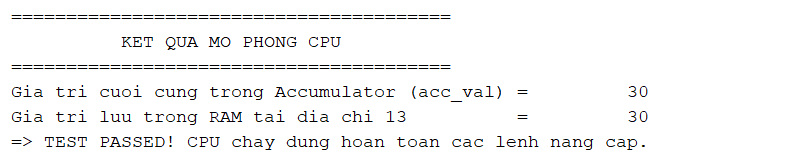
\includegraphics[width=0.8\textwidth]{console.png} 
    \caption{Kết quả Console mô phỏng hệ thống CPU nâng cao}
\end{figure}

\begin{quote}
    \textit{Giá trị cuối cùng trong Accumulator (\texttt{acc\_val}) = 30} \\
    \textit{Giá trị lưu trong RAM tại địa chỉ 13 = 30} \\
    \textbf{=> TEST PASSED! CPU chạy đúng hoàn toàn các lệnh nâng cấp.}
\end{quote}

Kết quả này khẳng định lệnh \textbf{STO} đã ghi thành công giá trị $30_{10}$ từ Accumulator vào địa chỉ 13 của bộ nhớ thông qua cơ chế bus dùng chung.
